% ----------------------------------------------------------------------
% Set the document class
% ----------------------------------------------------------------------
\documentclass[12pt]{article}

% ----------------------------------------------------------------------
% Packages
% ----------------------------------------------------------------------
\usepackage[utf8]{inputenc}
\usepackage[english]{babel}

\usepackage{booktabs}
\usepackage{listings}

\usepackage[export]{adjustbox}
\usepackage{amsmath}
\usepackage{amssymb}
\usepackage{anysize}
\marginsize{2cm}{2cm}{2cm}{2cm}

\usepackage{appendix}
\usepackage{cancel}

\usepackage{caption}
\captionsetup{labelfont={bf}}

\usepackage{cite}
\usepackage{color}

\usepackage{fancyhdr}
\pagestyle{fancy}
\fancyhf{}
\fancyhead[L]{\footnotesize IST}
\fancyhead[R]{\footnotesize ULisboa}
\fancyfoot[L]{\footnotesize Traffic Engineering}
\fancyfoot[C]{\thepage}
\fancyfoot[R]{\footnotesize METI}
\renewcommand{\footrulewidth}{0.4pt}

\usepackage{float}
\usepackage{graphicx}

\usepackage[
colorlinks = true,
plainpages = true,
linkcolor = istblue,
urlcolor = istblue,
citecolor = istblue,
anchorcolor = istblue
]{hyperref}

\usepackage{indentfirst}
\usepackage[super]{nth}
\usepackage{siunitx}
\usepackage{subcaption}
\usepackage{multirow}
\usepackage{titlesec}

\titleformat{\section}{\Large\bfseries}{\thesection}{1em}{}
\titleformat{\subsection}{\large\bfseries}{\thesubsection}{1em}{}
\titleformat{\subsubsection}{\normalsize\bfseries}{\thesubsubsection}{1em}{}

% Random text (not needed)
\usepackage{lipsum}
\usepackage{duckuments}

% ----------------------------------------------------------------------
% Commands
% ----------------------------------------------------------------------

\newcommand{\sen}{\operatorname{\sen}}
\newcommand{\HRule}{\rule{\linewidth}{0.5mm}}

% ----------------------------------------------------------------------
% Colors
% ----------------------------------------------------------------------

\definecolor{istblue}{RGB}{3,171,230}
\definecolor{dkgreen}{rgb}{0,0.6,0}
\definecolor{gray}{rgb}{0.5,0.5,0.5}

%%%%%%%%%%%%%%%%%%%%%%%%%%%%%%%%%%%%%%%%%%%%%%%%%%%%%%%%%%%%%%%%%%%%%%%%
% Document
%%%%%%%%%%%%%%%%%%%%%%%%%%%%%%%%%%%%%%%%%%%%%%%%%%%%%%%%%%%%%%%%%%%%%%%%

\begin{document}

% ----------------------------------------------------------------------
% Cover
% ----------------------------------------------------------------------

\begin{center}

\begin{figure}
    \vspace{-1.0cm}
    
\includegraphics[scale = 0.25, left]{Images/IST_A.png}
\end{figure}

\mbox{}\\[2.0cm]

\textsc{\Huge Traffic Engineering}\\[2.5cm]

\textsc{\LARGE METI}\\[2.0cm]

\HRule\\[0.4cm]

{\large \bf {Lab 2 Report} [\texttt{EN}]}\\[0.2cm]

\HRule\\[1.5cm]

\end{center}

\begin{flushleft}
\textbf{Authors:}
\end{flushleft}

\begin{center}

\begin{minipage}{0.5\textwidth}
\begin{flushleft}
José Oliveira (103771)\\
Tiago Videira (116069)\\
\end{flushleft}
\end{minipage}%
\begin{minipage}{0.5\textwidth}
\begin{flushright}
\href{mailto:jose.novais.oliveira@tecnico.ulisboa.pt}{\texttt{jose.novais.oliveira@tecnico.ulisboa.pt}}\\
\href{mailto:tiago.g.videira@tecnico.ulisboa.pt}{\texttt{tiago.g.videira@tecnico.ulisboa.pt}}\\
\end{flushright}
\end{minipage}

\end{center}

\begin{flushleft}
\large $\boxed{\text{\bf Group 5}}$\\[4.0cm]
\end{flushleft}

\begin{center}
\large \bf 2025/2026 -- \nth{2} Semester, P4
\end{center}

\thispagestyle{empty}

\setcounter{page}{0}

\tableofcontents

\newpage

% =========================================================
\section{Introduction}

The objective of this laboratory assignment was to implement and analyze IP routing mechanisms using Cisco routers within the GNS3 simulation environment.

The experiments performed throughout the laboratory focused on dynamic routing protocols, routing behavior, path selection mechanisms, and routing convergence.

The laboratory activities included:
\begin{itemize}
    \item IPv4 subnetting using VLSM;
    \item router interface configuration;
    \item OSPF routing configuration;
    \item routing table analysis;
    \item OSPF metric manipulation;
    \item connectivity verification;
    \item link failure simulation and convergence analysis.
\end{itemize}

The network topology consisted of five routers (R1 to R5) and two end devices (PC1 and PC2), interconnected through multiple redundant paths.

\newpage

% =========================================================
\section{Part A — OSPF Network Configuration}

% =========================================================
\subsection{Network Topology}

The network topology implemented in GNS3 is presented below.

\begin{figure}[H]
\centering
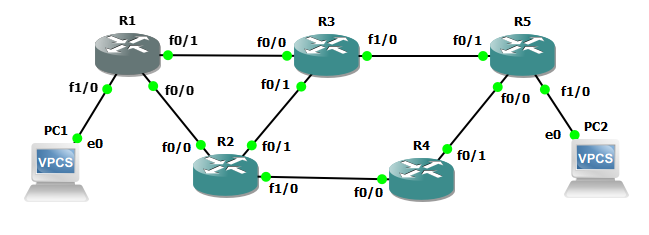
\includegraphics[width=0.85\textwidth]{../Topology-ETraf.PNG}
\caption{General network topology}
\end{figure}

The topology contains five routers interconnected through multiple redundant paths, allowing OSPF to dynamically calculate alternative routes in case of failures.

Additionally:
\begin{itemize}
    \item PC1 is connected to R1;
    \item PC2 is connected to R5.
\end{itemize}

% =========================================================
\subsubsection{Broadcast Domains}

Each physical link corresponds to an independent subnet/broadcast domain.

The network contains:
\begin{itemize}
    \item 6 router-to-router subnets;
    \item 2 LAN subnets (PC1-R1 and PC2-R5).
\end{itemize}

Therefore, the topology contains a total of:

\[
8 \text{ broadcast domains}
\]

\newpage
% =========================================================
\subsection{IPv4 Addressing Plan}

The network address block assigned was:

\[
192.168.5.0/24
\]

Using VLSM, the address space was segmented into multiple /30 subnets.

\begin{table}[H]
\centering
\begin{tabular}{ccc}
\toprule
\textbf{Link} & \textbf{Subnet} & \textbf{IPs Used} \\
\midrule
R1-R2 & 192.168.5.4/30 & .5 / .6 \\
R1-R3 & 192.168.5.8/30 & .9 / .10 \\
R2-R3 & 192.168.5.12/30 & .13 / .14 \\
R2-R4 & 192.168.5.16/30 & .17 / .18 \\
R4-R5 & 192.168.5.20/30 & .21 / .22 \\
R3-R5 & 192.168.5.24/30 & .25 / .26 \\
PC1-R1 & 192.168.5.0/30 & .1 / .2 \\
PC2-R5 & 192.168.5.28/30 & .29 / .30 \\
\bottomrule
\end{tabular}
\caption{IPv4 addressing plan}
\end{table}

% =========================================================
\subsection{Router Configuration}

Each router interface was configured manually.

Example configuration used on R1:

\begin{lstlisting}
interface FastEthernet1/0
ip address 192.168.5.2 255.255.255.252
no shutdown

interface FastEthernet0/0
ip address 192.168.5.5 255.255.255.252
no shutdown

interface FastEthernet0/1
ip address 192.168.5.9 255.255.255.252
no shutdown
\end{lstlisting}

The command below was used to verify interface status:

\begin{lstlisting}
show ip interface brief
\end{lstlisting}

All interfaces reached the \texttt{up/up} operational state.

The same configuration methodology was applied to all routers in the topology.

\newpage
% =========================================================
\subsection{OSPF Configuration}

OSPF was configured using process ID 1.

The following commands were applied:

\begin{lstlisting}
router ospf 1
network 192.168.5.0 0.0.0.255 area 0
\end{lstlisting}

After configuration, OSPF neighbor relationships were successfully established.

The command used to verify adjacency status was:

\begin{lstlisting}
show ip ospf neighbor
\end{lstlisting}

Routers reached the FULL adjacency state, confirming successful synchronization of OSPF databases.

All routers were configured within OSPF Area 0.

% =========================================================
\subsection{Routing Table Analysis}

The routing table was inspected using:

\begin{lstlisting}
show ip route
\end{lstlisting}

Routes learned dynamically through OSPF were identified with the letter:

\[
O
\]

Initially, multiple equal-cost paths existed for some destinations, demonstrating Equal Cost Multi-Path (ECMP) behavior.

Example:

\begin{lstlisting}
O 192.168.5.12 [110/20] via 192.168.5.10
                 via 192.168.5.6
\end{lstlisting}

This indicates that two paths with identical OSPF cost were available.

This demonstrated the capability of OSPF to support load balancing across equal-cost paths.

% =========================================================
\subsection{OSPF Cost Manipulation}

To analyze OSPF path selection behavior, the cost of interface FastEthernet0/1 on R1 was increased.

Configuration used:

\begin{lstlisting}
interface FastEthernet0/1
ip ospf cost 100
\end{lstlisting}

After modifying the cost:
\begin{itemize}
    \item OSPF recalculated the routing table;
    \item alternative lower-cost paths were selected;
    \item traffic was redirected automatically.
\end{itemize}

Traceroute confirmed the path modification.

Before: Equal-cost paths existed through both R2 and R3.

\[
R1 \rightarrow R2 \rightarrow R3 \rightarrow R5
\]

After: Traffic preferred the path through R2.
\[
R1 \rightarrow R3 \rightarrow R5
\]

This demonstrated OSPF metric-based path selection.

This experiment demonstrated how OSPF metrics directly influence path selection decisions.

% =========================================================
\subsection{Experimental Results}

This section presents the experimental results obtained during the implementation and testing of the network.

% ---------------------------------------------------------
\subsubsection{Interface Verification}

After configuring the interfaces, the following command was used to verify interface status:

\begin{lstlisting}
show ip interface brief
\end{lstlisting}

Example output from R1:

\begin{lstlisting}
Interface              IP-Address      Status      Protocol

FastEthernet0/0        192.168.5.5     up          up
FastEthernet0/1        192.168.5.9     up          up
FastEthernet1/0        192.168.5.2     up          up
\end{lstlisting}

The output confirmed that all interfaces were correctly configured and operational.

% ---------------------------------------------------------
\subsubsection{OSPF Neighbor Adjacency}

The following command was used to verify OSPF neighbor relationships:

\begin{lstlisting}
show ip ospf neighbor
\end{lstlisting}

Observed output:

\begin{lstlisting}
Neighbor ID     Pri   State      Dead Time   Address        Interface

192.168.5.25      1   FULL/BDR   00:00:32    192.168.5.10  FastEthernet0/1
192.168.5.17      1   FULL/DR    00:00:33    192.168.5.6   FastEthernet0/0
\end{lstlisting}

The FULL state confirmed that OSPF adjacencies were successfully established and routing databases were synchronized.

\newpage
% ---------------------------------------------------------
\subsubsection{Routing Table Analysis}

The routing table was analyzed using:

\begin{lstlisting}
show ip route
\end{lstlisting}

Example output:

\begin{lstlisting}
O 192.168.5.12 [110/20] via 192.168.5.10
                 via 192.168.5.6

O 192.168.5.24 [110/11] via 192.168.5.10

O 192.168.5.16 [110/11] via 192.168.5.6
\end{lstlisting}

Routes marked with the letter \texttt{O} correspond to routes learned through OSPF.

Initially, some routes had multiple equal-cost paths, demonstrating Equal Cost Multi-Path (ECMP) behavior.

% ---------------------------------------------------------
\subsubsection{OSPF Cost Manipulation}

To influence path selection, the OSPF cost of interface FastEthernet0/1 on R1 was increased.

Configuration used:

\begin{lstlisting}
interface FastEthernet0/1
ip ospf cost 100
\end{lstlisting}

After changing the cost, the routing table changed accordingly.

Updated routing example:

\begin{lstlisting}
O 192.168.5.12 [110/20] via 192.168.5.6

O 192.168.5.24 [110/21] via 192.168.5.6

O 192.168.5.20 [110/21] via 192.168.5.6
\end{lstlisting}

This confirmed that OSPF selected the path with the lowest accumulated metric.

% ---------------------------------------------------------
\subsubsection{Connectivity Verification}

Connectivity between end devices was tested using ICMP echo requests.

Command executed:

\begin{lstlisting}
ping 192.168.5.30
\end{lstlisting}

Observed output:

\begin{lstlisting}
!!!!!
Success rate is 100 percent (5/5)
\end{lstlisting}

This confirmed successful communication between PC1 and PC2.

Traceroute was also performed:

\begin{lstlisting}
traceroute 192.168.5.30
\end{lstlisting}

Observed route before OSPF cost manipulation:

\begin{lstlisting}
1 192.168.5.6
2 192.168.5.14
3 192.168.5.26
4 192.168.5.30
\end{lstlisting}

After increasing the OSPF cost, the selected route changed:

\begin{lstlisting}
1 192.168.5.10
2 192.168.5.26
3 192.168.5.30
\end{lstlisting}

This demonstrated successful dynamic route recalculation.

% ---------------------------------------------------------
\subsubsection{Link Failure and OSPF Convergence}

To evaluate convergence behavior, one of the active interfaces was disabled.

Command executed:

\begin{lstlisting}
interface FastEthernet0/0
shutdown
\end{lstlisting}

OSPF immediately detected the failure:

\begin{lstlisting}
%OSPF-5-ADJCHG:
Process 1, Nbr 192.168.5.17 on FastEthernet0/0
from FULL to DOWN
\end{lstlisting}

The routing table was automatically recalculated and traffic was redirected through alternative paths.

Traceroute after failure:

\begin{lstlisting}
1 192.168.5.10
2 192.168.5.26
3 192.168.5.30
\end{lstlisting}

The interface was restored using:

\begin{lstlisting}
no shutdown
\end{lstlisting}

OSPF adjacency was re-established successfully:

\begin{lstlisting}
%OSPF-5-ADJCHG:
Process 1, Nbr 192.168.5.17
from LOADING to FULL
\end{lstlisting}

This demonstrated:
\begin{itemize}
    \item automatic fault detection;
    \item dynamic rerouting;
    \item successful OSPF convergence.
\end{itemize}

\newpage

\section{Part B — MPLS Configuration and Analysis}

\subsection{Introduction}

The objective of Part B was to configure and analyze an MPLS-based network using Cisco routers in GNS3.

The experiments focused on:
\begin{itemize}
    \item enabling MPLS forwarding;
    \item configuring LDP (Label Distribution Protocol);
    \item analyzing MPLS forwarding tables;
    \item observing MPLS labels using Wireshark;
    \item demonstrating Penultimate Hop Popping (PHP);
    \item testing MPLS recovery after link failures.
\end{itemize}

The MPLS network was implemented on top of the OSPF infrastructure configured in Part A.

% =========================================================
\subsection{MPLS Configuration}

Cisco Express Forwarding (CEF) was enabled on all routers to support MPLS operation.

The following commands were applied:

\begin{lstlisting}
ip cef
mpls ip
\end{lstlisting}

MPLS was enabled on the router interfaces participating in the MPLS core.

Example configuration on R3:

\begin{lstlisting}
interface FastEthernet0/0
mpls ip

interface FastEthernet1/0
mpls ip

interface FastEthernet1/1
mpls ip
\end{lstlisting}

OSPF was used as the underlying routing protocol to distribute reachability information between routers.

% =========================================================
\subsection{LDP Neighbor Verification}

LDP neighbors were verified using the following command:

\begin{lstlisting}
show mpls ldp neighbor
\end{lstlisting}

Example output obtained on R3:

\begin{lstlisting}
Peer LDP Ident: 192.168.5.9:0
State: Oper

Peer LDP Ident: 192.168.5.29:0
State: Oper

Peer LDP Ident: 192.168.5.17:0
State: Oper
\end{lstlisting}

The \texttt{Oper} state confirmed that LDP sessions were successfully established and labels were being exchanged between MPLS routers.

% =========================================================
\subsection{MPLS Interface Verification}

MPLS-enabled interfaces were verified using:

\begin{lstlisting}
show mpls interfaces
\end{lstlisting}

Example output:

\begin{lstlisting}
Interface              IP            Operational
FastEthernet0/0        Yes (ldp)     Yes
FastEthernet1/0        Yes (ldp)     Yes
FastEthernet1/1        Yes (ldp)     Yes
\end{lstlisting}

This confirmed that MPLS forwarding and LDP were operational on all core links.

% =========================================================
\subsection{MPLS Forwarding Table Analysis}

The MPLS forwarding table was inspected using:

\begin{lstlisting}
show mpls forwarding-table
\end{lstlisting}

Example output obtained on R3:

\begin{lstlisting}
Local  Outgoing  Prefix
Label  Label

16     Pop Label 192.168.5.4/30
17     Pop Label 192.168.5.0/30
18     Pop Label 192.168.5.16/30
19     Pop Label 192.168.5.20/30
20     Pop Label 192.168.5.28/30
\end{lstlisting}

The forwarding table demonstrated that MPLS labels were correctly assigned and distributed across the network.

The presence of the \texttt{Pop Label} operation confirmed the implementation of Penultimate Hop Popping (PHP).

% =========================================================
\subsection{Wireshark Analysis and PHP Demonstration}

Wireshark captures were performed to analyze MPLS label switching behavior.

Traffic was generated using:

\begin{lstlisting}
ping 192.168.5.30
\end{lstlisting}

and:

\begin{lstlisting}
trace 192.168.5.30
\end{lstlisting}

% ---------------------------------------------------------
\subsubsection{MPLS Labels in the Core Network}

Wireshark captures performed on core MPLS links showed packets containing MPLS headers.

The captured packets contained entries similar to:

\begin{lstlisting}
MultiProtocol Label Switching Header
Label: 20
\end{lstlisting}

This confirmed that MPLS labels were being attached and switched correctly inside the MPLS core.

\begin{figure}[H]
\centering
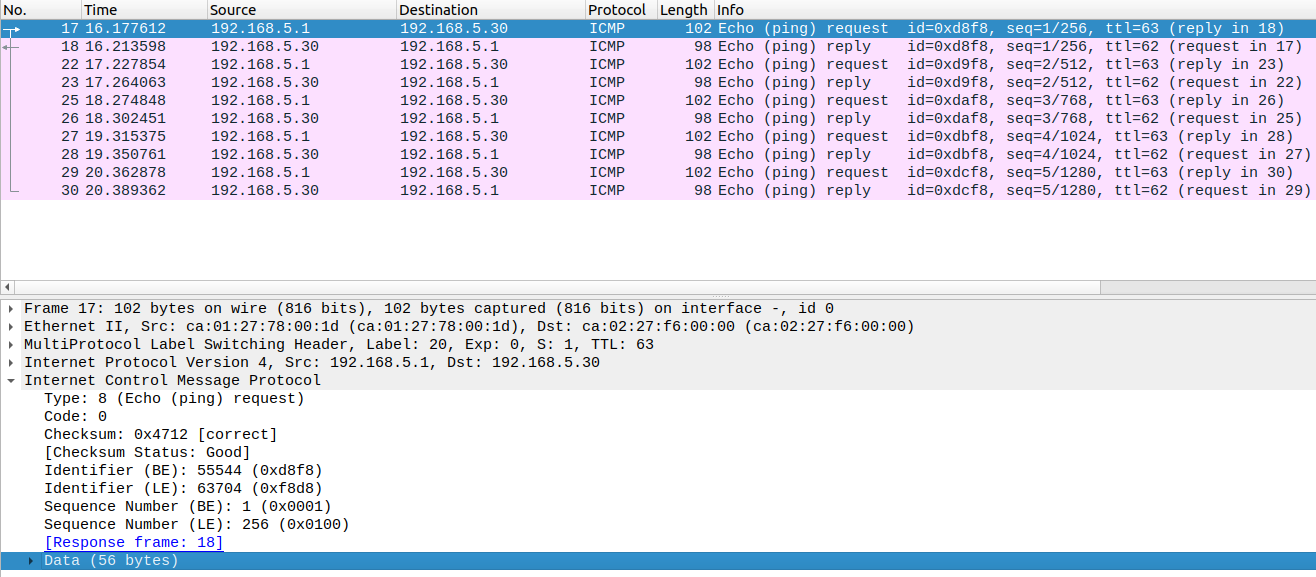
\includegraphics[width=0.9\textwidth]{../MPLS_Label_Core.png}
\caption{MPLS labeled packet captured in the MPLS core}
\end{figure}

% ---------------------------------------------------------
\subsubsection{Penultimate Hop Popping (PHP)}

Additional captures were performed on the final hop between R5 and PC2.

The captured packets no longer contained MPLS headers and only displayed IP and ICMP information.

This demonstrated that the MPLS label was removed by the penultimate router before reaching the egress router.

Therefore, Penultimate Hop Popping (PHP) was successfully verified.

\begin{figure}[H]
\centering
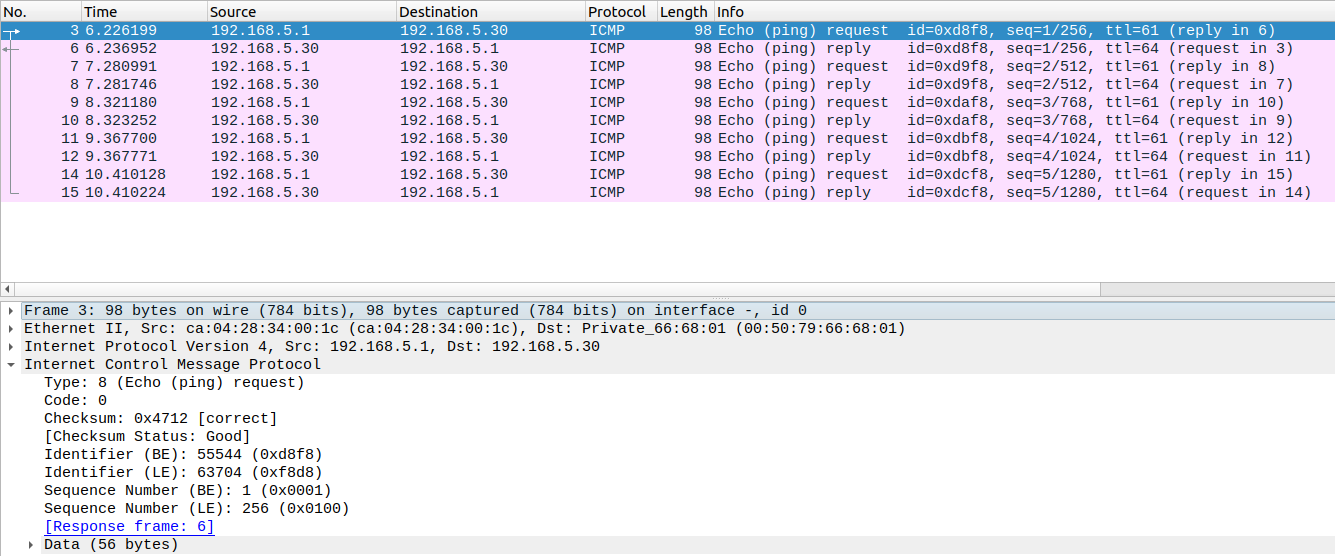
\includegraphics[width=0.9\textwidth]{../PHP_No_Label.png}
\caption{Packet capture after PHP operation (no MPLS label present)}
\end{figure}

% =========================================================
\subsection{Connectivity Verification}

Connectivity between PC1 and PC2 was verified using ICMP echo requests.

The following command was executed:

\begin{lstlisting}
ping 192.168.5.30
\end{lstlisting}

Observed output:

\begin{lstlisting}
!!!!!
Success rate is 100 percent (5/5)
\end{lstlisting}

This confirmed successful MPLS forwarding and end-to-end connectivity.

Traceroute was also performed:

\begin{lstlisting}
trace 192.168.5.30
\end{lstlisting}

Observed route before link failure:

\begin{lstlisting}
1 192.168.5.2
2 192.168.5.10
3 192.168.5.26
4 192.168.5.30
\end{lstlisting}

This path corresponded to:

\[
R1 \rightarrow R3 \rightarrow R5
\]

% =========================================================
\subsection{MPLS Failure Recovery and Convergence}

To evaluate MPLS recovery behavior, the primary MPLS path between R1 and R3 was disabled.

The following command was applied on R1:

\begin{lstlisting}
interface FastEthernet1/1
shutdown
\end{lstlisting}

After the failure:
\begin{itemize}
    \item OSPF recalculated the routing table;
    \item LDP sessions were updated;
    \item MPLS forwarding switched to an alternative LSP.
\end{itemize}

Traceroute after the failure produced the following output:

\begin{lstlisting}
1 192.168.5.2
2 192.168.5.6
3 192.168.5.14
4 192.168.5.26
5 192.168.5.30
\end{lstlisting}

The new path corresponded to:

\[
R1 \rightarrow R2 \rightarrow R3 \rightarrow R5
\]

This demonstrated successful MPLS rerouting and network resilience after link failure.

The failed interface was restored using:

\begin{lstlisting}
interface FastEthernet1/1
no shutdown
\end{lstlisting}

After convergence, the original LSP was automatically restored.

% =========================================================
\subsection{Conclusion}

This part of the laboratory successfully demonstrated the deployment and operation of MPLS forwarding in a Cisco-based network.

The experiments confirmed:
\begin{itemize}
    \item successful LDP neighbor establishment;
    \item MPLS label distribution and forwarding;
    \item operation of Penultimate Hop Popping (PHP);
    \item MPLS traffic analysis using Wireshark;
    \item MPLS recovery after link failures.
\end{itemize}

The obtained results demonstrated the robustness and flexibility of MPLS networks under dynamic routing conditions.

Overall, the laboratory provided practical experience with MPLS forwarding, label switching, and traffic engineering concepts.

\newpage


\newpage
% =========================================================
\section{Conclusion}

This laboratory assignment successfully demonstrated the deployment and analysis of an OSPF-based IP network using Cisco routers in GNS3.

The implementation of VLSM enabled efficient IPv4 address allocation across all network segments. OSPF dynamically exchanged routing information and automatically selected optimal paths according to interface metrics.

Several experiments were performed to evaluate OSPF behavior under different network conditions, including:
\begin{itemize}
    \item routing table analysis;
    \item OSPF cost manipulation;
    \item connectivity verification;
    \item link failure simulation;
    \item routing convergence analysis.
\end{itemize}

The obtained results demonstrated:
\begin{itemize}
    \item successful end-to-end connectivity;
    \item dynamic path recalculation;
    \item automatic failover capabilities;
    \item fast OSPF convergence.
\end{itemize}

Overall, this assignment provided practical experience with dynamic routing protocols and fundamental traffic engineering concepts.

\end{document}